\documentclass{article}

%% Page Margins %%
\usepackage{geometry}
\geometry{
    top = 0.75in,
    bottom = 0.75in,
    right = 0.75in,
    left = 0.75in,
}

\usepackage{amsmath}
\usepackage{graphicx}
\usepackage{parskip}

\title{Assembly Project: Dr Mario}

\author{Bhavya Jain}

\begin{document}
\maketitle

\section{Instruction and Summary}

\begin{enumerate}

    \item Which milestones were implemented? 
        \begin{itemize}
            \item Milestone 1
            \item Milestone 2
            \item Milestone 3
            \item Milestone 4 and Milestone 5 (1 Hard, 6 Easy)
            \begin{itemize}
                \item Easy
                \begin{enumerate}
                    \item Implemented Gravity (1)
                    \item Increasing Gravity speed over time (2)
                    \item Game Over and Retry (4)
                    \item Sound effects when moving capsule, rotating capsule, and      
                     game over (5)
                     \item Pause functionality with display (6)
                     \item Draw Dr. Mario and the viruses

                \end{enumerate}
                \item Hard
                \end{itemize}
                \begin{itemize}
                    \item Background Music
                \end{itemize}
        \end{itemize}

    \item How to view the game:
    
    \begin{enumerate}

    \item1 unit
    \item64 width
    \item128 height


    \end{enumerate}

    

\begin{figure}[ht!]
    \centering
     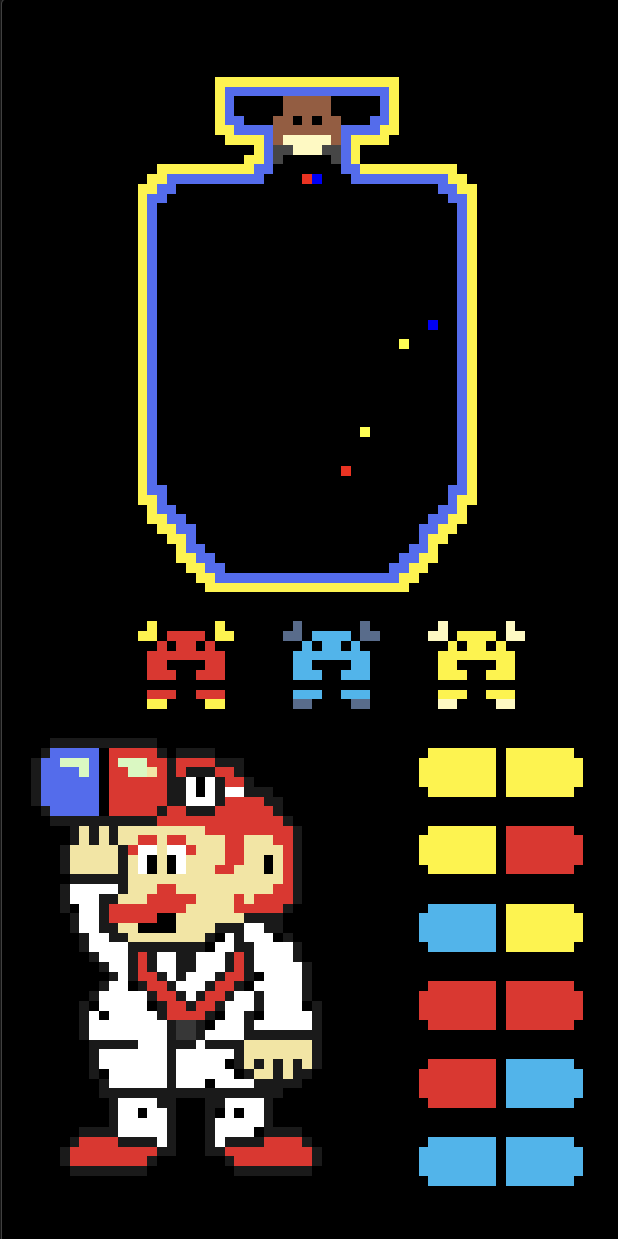
\includegraphics[width=0.3\textwidth]{game.png}
    \caption{Dr Mario 4K UHD}
    \label{Dr Mario}
\end{figure}

\item Game Summary:
% TODO: Tell us a little about your game.
\begin{itemize}
\item Controls: WASD for movement (left, rotate, down, right), P to pause, Q to quit, R to restart
\item Graphics created on pixilart.org using game references, then converted to MIPS data points using custom Python scripts
\item Attempted to draw a Goomba at the top of the medicine bottle (limited by display resolution)
\item Dr. Mario sprite has ginger hair and some colors differ from original game due to colorblindness
\item  All music implemented by converting MIDI file into component arrays (duration, timing, velocity, instrument) to be played via MIPS syscalls
\item Display configured as 64x128 pixels (1 pixel per unit) with base address 0x10008000
\end{itemize}

    
\end{enumerate}

\section{Attribution Table}
% TODO: If you worked in partners, tell us who was 
%       responsible for which features. Some reweighting 
%       might be possible in cases where one group member
%       deserves extra credit for the work they put in.
Project was done solo



\end{document}